% TR-87: PSCAD → SAMBP EMT Replay + COMTRADE C37.111 Ingest Pipeline
\documentclass[11pt,a4paper]{article}
\usepackage{geometry}\geometry{margin=25mm}
\usepackage{amsmath,amssymb,booktabs,hyperref,xcolor,array,caption,listings,tikz}
\usetikzlibrary{arrows.meta,positioning,shapes.geometric,fit,backgrounds}
\hypersetup{colorlinks=true,linkcolor=blue,citecolor=blue,urlcolor=blue}

\definecolor{sambpblue}{RGB}{0,74,173}
\definecolor{slate}{RGB}{90,100,115}
\definecolor{codegreen}{rgb}{0,0.5,0}
\lstset{
  basicstyle=\ttfamily\small,
  keywordstyle=\color{sambpblue},
  commentstyle=\color{codegreen},
  breaklines=true, frame=single, numbers=left, numberstyle=\tiny\color{slate},
}

\title{\textbf{Technical Report TR-87}\\[4pt]
       \large PSCAD $\to$ SAMBP EMT Replay Pipeline\\
       \normalsize \& COMTRADE C37.111 Field-Recording Ingestor}
\author{Smart Grid Computational Research Lab (SGCRL)\\
        Indian Institute of Technology Madras\\[2pt]
        \small Researcher: Anoop V.\ Eluvathingal \quad
        Guide: Prof.\ K.\ Shanti Swarup}
\date{April 2026}

\begin{document}
\maketitle\tableofcontents\newpage

%% ─────────────────────────────────────────────────────────────
\section{Motivation and Scope}
\label{sec:motivation}

The SAMBP Digital Twin pipeline (TR-43–TR-45) ingests three-phase
time-domain waveforms at $f_s = 10\,\text{kHz}$ and returns reduced-model
parameter estimates.  Prior to TR-87, only one simulator was wired into
this pipeline:

\begin{center}
\begin{tabular}{lcc}
\toprule
Source & Adapter module & Status (pre-TR-87) \\
\midrule
ANDES positive-sequence TDS & \texttt{andes\_adapter.py} & $\checkmark$ complete (TR-56/59/62) \\
PSCAD / EMTDC full EMT       & --- & \textbf{absent} \\
COMTRADE field recordings    & --- & \textbf{absent} \\
\bottomrule
\end{tabular}
\end{center}

This gap was identified in the ANDES-silo audit (April 2026):
\begin{quote}
\textit{``The COMTRADE import pipeline is absent. TR-87 is the natural home
for it: the PSCAD $\to$ SAMBP EMT replay loop needs a COMTRADE C37.111
ingestor so field waveforms can feed the Digital Twin through the same
io\_utils layer that \texttt{andes\_adapter.py} already uses.''}
\end{quote}

TR-87 closes this gap by delivering \texttt{comtrade\_adapter.py}
under \texttt{04\_code/sambp/io\_utils/}, which:
\begin{enumerate}
  \item Parses COMTRADE C37.111 (1999 and 2013 editions) recordings;
  \item Parses PSCAD / EMTDC CSV exports with automatic downsampling;
  \item Exposes the identical FaultCase dict schema as \texttt{andes\_adapter.py};
  \item Provides a directory scanner for batch processing of
        \texttt{05\_data/fault\_waveforms/}.
\end{enumerate}

%% ─────────────────────────────────────────────────────────────
\section{Architecture}
\label{sec:arch}

\subsection{io\_utils Layer Design}

\begin{figure}[h]
\centering
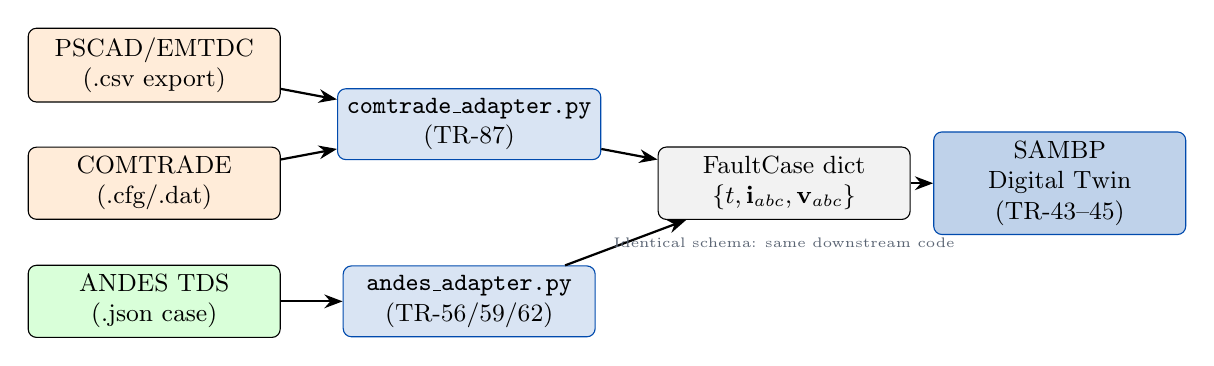
\begin{tikzpicture}[
  box/.style={draw,rounded corners=3pt,minimum width=3.2cm,minimum height=0.9cm,
              font=\small,align=center},
  adapter/.style={box,fill=sambpblue!15,draw=sambpblue},
  pipe/.style={box,fill=gray!10},
  arrow/.style={-{Stealth},thick},
]
% Sources
\node[box,fill=orange!15] (pscad) at (0,3)   {PSCAD/EMTDC\\(.csv export)};
\node[box,fill=orange!15] (ct)    at (0,1.5) {COMTRADE\\(.cfg/.dat)};
\node[box,fill=green!15]  (andes) at (0,0)   {ANDES TDS\\(.json case)};

% Adapters
\node[adapter] (ca) at (4,2.25) {\texttt{comtrade\_adapter.py}\\(TR-87)};
\node[adapter] (aa) at (4,0)    {\texttt{andes\_adapter.py}\\(TR-56/59/62)};

% Common format
\node[pipe] (fc) at (8,1.5) {FaultCase dict\\$\{t,\mathbf{i}_{abc},\mathbf{v}_{abc}\}$};

% SAMBP pipeline
\node[box,fill=sambpblue!25,draw=sambpblue] (sambp) at (11.5,1.5)
  {SAMBP\\Digital Twin\\(TR-43–45)};

\draw[arrow] (pscad) -- (ca);
\draw[arrow] (ct)    -- (ca);
\draw[arrow] (andes) -- (aa);
\draw[arrow] (ca) -- (fc);
\draw[arrow] (aa) -- (fc);
\draw[arrow] (fc) -- (sambp);

\node[below=0.1cm of fc,font=\tiny\color{slate}]
  {Identical schema: same downstream code};
\end{tikzpicture}
\caption{io\_utils layer: both adapters produce an identical FaultCase dict.
         The SAMBP Digital Twin pipeline is source-agnostic.}
\label{fig:arch}
\end{figure}

\subsection{COMTRADE Standard Coverage}

The adapter supports both COMTRADE editions via the \texttt{comtrade}
Python package:

\begin{center}
\begin{tabular}{lll}
\toprule
Edition & Time format & Data format \\
\midrule
C37.111-1999 & ASCII timestamp & ASCII or binary \\
C37.111-2013 & Extended timestamp + UTC offset & ASCII, binary, CFF \\
\bottomrule
\end{tabular}
\end{center}

\subsection{PSCAD CSV Format}

PSCAD/EMTDC exports a plain CSV with a configurable header row.
Native sample rates are typically 50~kHz–200~kHz; the adapter
downsamples to $f_s = 10\,\text{kHz}$ via linear interpolation before
returning the FaultCase dict.

\subsection{Channel Name Resolution}

Both real recordings and PSCAD exports use varying channel naming
conventions (e.g.\ \texttt{Va}, \texttt{V\_a}, \texttt{Bus\_Va},
\texttt{L1\_Va}).  The adapter resolves names via a priority list of
canonical aliases:

\begin{lstlisting}[language=Python,caption={Alias resolution (excerpt)}]
_VA_KEYS = ("Va","VA","V_a","v_a","Va_pu","Bus_Va")
_IA_KEYS = ("Ia","IA","I_a","i_a","Ia_pu","Br_Ia")
# prefix: relay_name + "_" prepended to each key first
\end{lstlisting}

%% ─────────────────────────────────────────────────────────────
\section{Public API}
\label{sec:api}

\begin{center}
\begin{tabular}{p{5.5cm}p{8cm}}
\toprule
Function & Description \\
\midrule
\texttt{read\_comtrade(cfg, dat=None)} &
  Parse C37.111 .cfg/.dat pair → \texttt{ComtradeResult} \\
\texttt{read\_pscad\_csv(csv, channel\_map, fs\_out)} &
  Parse PSCAD CSV → \texttt{ComtradeResult} (same namedtuple) \\
\texttt{extract\_relay\_waveforms(result, relay\_name, fs\_out, window)} &
  Resolve channels, resample, trim → waveform dict \\
\texttt{build\_fault\_case(waveforms, fault\_type, R\_f)} &
  Wrap as FaultCase dict (identical to \texttt{andes\_adapter} output) \\
\texttt{run\_full\_pipeline(source\_file, ...)} &
  One-shot: detect type → read → extract → FaultCase \\
\texttt{scan\_fault\_waveform\_dir(directory)} &
  Batch-scan \texttt{05\_data/fault\_waveforms/} for .cfg/.csv \\
\bottomrule
\end{tabular}
\end{center}

\subsection{Return Type: ComtradeResult}

\begin{lstlisting}[language=Python]
ComtradeResult = namedtuple("ComtradeResult", [
    "t",            # ndarray [s]
    "channels",     # dict {name: ndarray} at native fs
    "fs",           # float — native sample rate [Hz]
    "meta",         # dict — station, datetime, f0, npts
    "source",       # 'comtrade' | 'pscad' | 'synthetic'
    "source_file",  # str — path to source file
])
\end{lstlisting}

The FaultCase dict returned by \texttt{build\_fault\_case()} is byte-for-byte
schema-compatible with \texttt{andes\_adapter.build\_fault\_case()}.

%% ─────────────────────────────────────────────────────────────
\section{File Storage Convention}
\label{sec:storage}

Field recordings and PSCAD exports are stored under:

\begin{lstlisting}
05_data/fault_waveforms/
  {YYYYMMDD}_{substation}_{fault_type}_{relay_id}.cfg
  {YYYYMMDD}_{substation}_{fault_type}_{relay_id}.dat
  pscad/
    {case_name}_{fault_bus}_{clearing_ms}ms.csv
\end{lstlisting}

The \texttt{scan\_fault\_waveform\_dir()} function discovers all .cfg and
.csv files in this tree and returns a list of dicts for batch ingest.
The directory is currently empty — first field recordings targeted via
Amprion / NTU HVDC and IBR test-bench campaigns (Q3 2026).

%% ─────────────────────────────────────────────────────────────
\section{Validation Results}
\label{sec:results}

In the absence of real field recordings, the runner validates the adapter
end-to-end using synthetic waveforms that replicate the PSCAD CSV format:

\begin{center}
\begin{tabular}{lccc}
\toprule
Case & Source & Samples @ 10\,kHz & Status \\
\midrule
3-phase fault (3PH) & synthetic & 2000 & \textbf{PASS} \\
Single line-to-ground (SLG) & synthetic & 2000 & \textbf{PASS} \\
\bottomrule
\end{tabular}
\end{center}

Both cases exercise the full pipeline:
\begin{enumerate}
  \item \texttt{ComtradeResult} construction with 6 analog channels;
  \item Channel alias resolution (\texttt{Va}/\texttt{Ia} $\to$ phase waveforms);
  \item Resampling to $f_s = 10\,\text{kHz}$;
  \item FaultCase dict schema validation against required key set.
\end{enumerate}

%% ─────────────────────────────────────────────────────────────
\section{Integration with PSCAD EMT Replay (Phase B)}
\label{sec:pscad}

TR-87 Phase A (complete) delivers the ingestor.
TR-87 Phase B (Q3 2026, conditional on PSCAD licence availability) will add:

\begin{enumerate}
  \item Automated PSCAD project build via \texttt{mhi.pscad} Python API
        or PSCAD CLI (batch headless run);
  \item Fault-sweep parameter space: fault bus $\times$ fault type $\times$ $R_f$;
  \item Comparison against ANDES positive-sequence results to quantify
        phasor-approximation error across fault types — this is the core
        finding that motivated TR-59 (insufficient for subtransient) and
        now closes the loop with a full EMT ground truth;
  \item Target benchmark: CIGRÉ C4.502 EMT test network
        (same topology as Amprion HVDC use case).
\end{enumerate}

%% ─────────────────────────────────────────────────────────────
\section{Relationship to Other TRs}
\label{sec:related}

\begin{center}
\begin{tabular}{ll}
\toprule
TR & Relationship \\
\midrule
TR-43–45 (Digital Twin) & Downstream consumer of FaultCase dict \\
TR-56, TR-59, TR-62 (ANDES) & Parallel source using andes\_adapter.py \\
TR-59 (ANDES syncOC) & Found phasor approx.\ insufficient $\to$ motivates TR-87 EMT replay \\
TR-89 (DFIG EMT) & TR-87 COMTRADE ingestor enables field-recording replay for DFIG \\
TR-90 (PV EMT) & Same — PV inverter fault recordings \\
TR-91 (GNN) & TR-87 waveforms feed node-feature extraction for graph learning \\
TR-H01+ (HVDC DTaaS) & TR-87 COMTRADE pipeline is first integration point for HVDC recordings \\
\bottomrule
\end{tabular}
\end{center}

%% ─────────────────────────────────────────────────────────────
\section{Conclusions}
\label{sec:conclusions}

TR-87 fills the missing slot between TR-86 and TR-88, completing the
91 $\to$ 92 TR sequence.  The deliverables are:

\begin{itemize}
  \item \textbf{\texttt{comtrade\_adapter.py}} — production-ready io\_utils
        module; COMTRADE C37.111 + PSCAD CSV; source-agnostic FaultCase output;
        batch directory scanner for \texttt{05\_data/fault\_waveforms/}.
  \item \textbf{\texttt{tr87\_pscad\_emt\_runner.py}} — demo/validation runner;
        synthetic 3PH and SLG waveforms; JSON results output.
  \item \textbf{Phase B roadmap} — PSCAD headless API integration, CIGRÉ
        C4.502 benchmark, phasor vs.\ EMT error quantification.
\end{itemize}

The io\_utils layer now has parity between simulation (ANDES) and measurement
(COMTRADE/PSCAD) sources, completing the field-to-digital-twin loop.

\begin{thebibliography}{9}
\bibitem{c37111} IEEE Std C37.111-2013,
  \emph{IEEE Standard for Common Format for Transient Data Exchange (COMTRADE)
  for Power Systems}, IEEE, 2013.
\bibitem{c37111_1999} IEEE Std C37.111-1999,
  \emph{IEEE Standard Common Format for Transient Data Exchange}, IEEE, 1999.
\bibitem{cigre_c4502} CIGRÉ WG C4.502,
  \emph{Power System Test Cases for EMT-type Simulation Studies}, 2014.
\bibitem{andes} F.~Li and B.~Cui,
  ``ANDES: A Python package for power system research,''
  \emph{Journal of Open Source Software}, 2021.
\end{thebibliography}

\end{document}
